\chapter{The game Tichu}

\begin{figure}[ht]
    \begin{center}
        \begin{subfigure}[h]{.3\textwidth}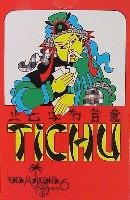
\includegraphics[width=\textwidth]{images/tichu_box}\end{subfigure}~
        \begin{subfigure}[h]{.5\textwidth}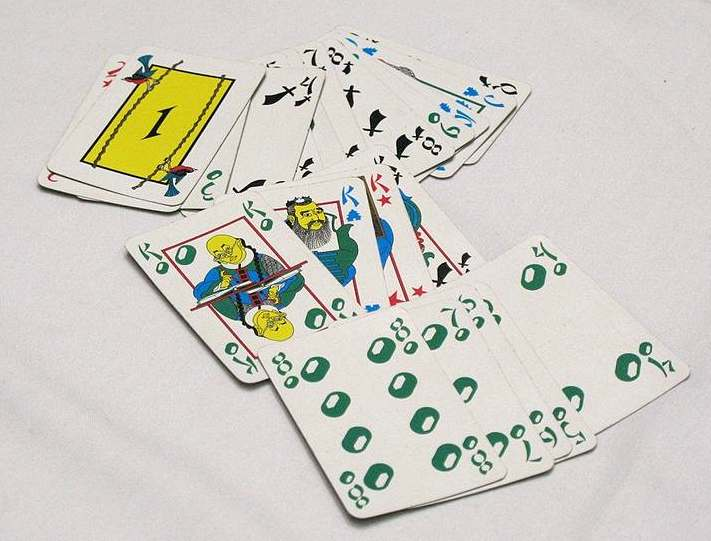
\includegraphics[width=\textwidth]{images/Tichu_cards}\end{subfigure}
    \end{center}
    \caption[Tichu the game]{Pictures of the game and cards}
\end{figure}
Tichu is a 4-player gambling card game which is marketed by Fata-Morgana \cite{fatamorgana}. It falls into the category of ladder games, where players must play a "higher" ranked set of cards on their turn or pass. The four players build 2 teams which compete against each other for points.
Tichu contains elements from some Chinese card-games such as \textit{Dou Di Zhu} or \textit{Zheng Fen} and is very popular in the german part of Switzerland.

\section{Rules}
More detailed rules can be found in \cite{fatamorgana, rules}.\\
The game is played in successive rounds until one team reaches a predefined amount of points.

\noindent\textbf{Cards} \\
There are 4 suits (Sword, Pagoda, Star, Jade) of 13 cards each corresponding in rank to the standard Bridge cards (2, 3, ... ,10, J, Q, K, A). In addition there are 4 special cards without any suit: \textit{Mah-Jong, Dog, Phoenix} and \textit{Dragon}. Hence there are 56 cards in total.

\noindent\textbf{Preparation}\\
The winner of the previous round shuffles and cuts the deck. When all cards are distributed, each player gives one card to each of the 3 other players. This phase is called card trading.

\noindent\textbf{The Game}\\
A round is started by the player who has the \textit{Mah-Jong} card. He may lay down any one of the following combinations:
\begin{description}
    \item[Single] A single card
    \item[Pair] Two cards of the same rank
    \item[Triple] Three cards of the same rank
    \item[Square] Four cards of the same rank
    \item[Fullhouse] A triple and pair together
    \item[Straight] At least five cards of consecutive ranks
    \item[Pair Step] Two or more consecutive Pairs (ie, J, J, Q, Q, A, A)
\end{description}

The next player (on the right) has two options, either to play a combination of the same type but with a higher rank, or to pass (not play at all). That means, for example, a pair can only be beaten by another pair of strictly higher rank and a straight only by another, higher straight of the same length.\\
The play then proceeds to the next player. If all players pass consecutively the trick ends and the player who laid the last combination takes the trick and leads a new one. If he has no more hand-cards, he retires from the game and the next not-retired player may start the trick.

\textbf{Bombs} \\
Bombs are either a straight where all cards have the same suit ("straight flush") or four cards of the same rank ("square").
A bomb beats all other combinations and a higher bomb beats a lower one. Any straight bomb is higher than a square bomb and a longer straight bomb beats a shorter one.
Bombs can be played at any time during a trick but only after the first play was made.

\textbf{The Special Cards}\\
\textit{Mah-Jong:} Whoever has this cards makes the first lead. The \textit{Mah-Jong} has a rank of 1 and can be used in a straight (eg. 1,2,3,4,5,6).
When a player plays the \textit{Mah-Jong}, he can wish any specific card rank (not including special cards). The next player who has a card with the wished rank and can play it \textit{in accordance with the rules of the game}, must play it. This condition remains in force until somebody plays such a card.

\noindent \textit{Dog:} The dog has no rank and can only be played as single card and only as \textit{first-play} (first card of a new trick). It immediately gives the lead to the partner of the player who played the dog (it can't be beaten by a bomb). If the partner already finished (has no handcards left) then the lead passes to the player on the right.

\noindent \textit{Dragon:} The dragon is the highest single card and can also only be played as a single card. If the Dragon wins the trick, the player must give the entire trick to any player of the opposing team.

\noindent \textit{Phoenix:} The phoenix can be used as a joker in any combination but it can't be used to create a bomb. It also can't replace any other special card.
When played as a single card it has a value half a point above the last played card but it can't beat the dragon. If it is played first it has a value of 1.5.

\noindent\textbf{Calling Tichu}\\
Before playing his first card, each player has the right to announce a "Tichu". If he then wins the round (finishes first), his team receives 100 additional points - otherwise the team loses 100 points.
A player can also announce a "grand Tichu" before getting the $9^{th}$ card from the dealer. This gives 200 additional points (in case of success) or a penalty of -200 otherwise.\\

\noindent\textbf{Goal of the game}\\
The round is played until three of the four players have played all of their cards.
The remaining player gives his remaining handcards to the opposing team and all the tricks he won to the player who finished first.
% TODO tichu points
Then the cards of each team are counted as follows:
\begin{itemize}
    \item Kings and 10's are worth 10 points each
    \item 5's are 5 points each
    \item The Dragon is worth 25 points
    \item The Phoenix costs 25 points (is worth \textbf{-}25)
\end{itemize}

However, if both players of the same team have a doublewin (both finished before any of the opposing team), then that team gets 200 points and the card points are not counted.

When one team reaches a predefined number of points (usually 1000) they are the winners of the game.


\section{Tactics}
\label{sec:tactics}
Beginners are often told to concentrate on finishing first and not to pay attention on at the points of the cards during the game. This is good advice and even advanced players don't pay too much attention to the actual point-values of the cards when considering to play a combination. \newline
Getting rid of cards in ascending order is already a good strategy as having low card at the end makes it quite hard to finish. That said, it is seldom advantageous to split combinations apart.

Team-play is key. Points won by announcing Tichu and from doublewins often dominate points won with tricks during the game.
It is therefore extremely important to support your partner when she announced a Tichu and an enemy Tichu or doublewin should be prevented at all cost.

This is not a comprehensive list of tactics by any mean, but it helps to get a better idea of the game.


\section{Tichu and Artificial Intelligence}
Tichu is quite different from "classical" games such as chess or Connect Four.

First of all, it is a game with hidden information since the handcards of the other players are unknown (with the exception of the traded cards at the beginning). This introduces several problems discussed in the section \textit{\nameref{par:hiddeninfo}} below.\\
The second big difference to the classical games is that the game is both, a cooperative and competitive at the same time. In a team the players must play cooperatively and help each other while competing with the other team for points.\\
Tichu is a deterministic game in the sense that the effect of each action is known with certainty. However, it is not possible to determine precisely what the possible actions of any of the other players may be since their handcards are not known. This makes is necessary to model Tichu as a stochastic game from the viewpoint of a player.\\
The game is played over several, in essence independent, rounds which makes it an episodic game. Each round consists of several tricks being played, so each round has also an episodic nature. However, unlike the rounds, the tricks of the same round are not independent. The actions in a trick depend on actions played in previous ones.\\
Tichu is a discrete, turn based game. The fact that bombs can be played at any time can be modeled with a 'fast round': After each played combination all players have to decide whether they want to play a bomb or not. Then, the next player can play a 'normal' combination.\\
Finally, Tichu is a zero-sum game even though the points of a round typically don't sum up to zero. At the end exactly one team wins, the other looses. It is possible to center the points after each round around zero to make them sum up to zero without impacting the gameplay at all.

\subsection{Difficulties}
 Tichu is in several aspects a "difficult" game for AI.
 In this section some of the difficulties are presented.

\paragraph{Hidden Information}
\label{par:hiddeninfo}
The problem with games with hidden information is that a player does not have all information necessary to find the optimal action. This leads to uncertainty about "how good" each action actually is since it depends, at least partially, on the hidden information (or else the game is probably not fun to play). In most such games it is a big advantage to learn or at least approximate the hidden information, Tichu is no exception. \\
A player knowing exactly what the other players handcards are can determine the best action with 100\% confidence. However, due to the random dealing of the cards, knowing everything doesn't guarantee a win. It may happen that the enemy just has better cards. This implies that perfect information might not be as important in Tichu as in other games.\\ % TODO better übergang
There are roughly two different approaches to deal with hidden information. Infer the information, for example from the way a player plays, or deal with it by finding out what actions are good in a lot of possible cases.
This project explores both approaches to a certain degree.

\paragraph{Big branching factor}
\label{par:branchingfactor}
Even without the hidden information Tichu would be challenging, not least because of the large branching factor of the gametree\footnote{for gametree see \ref{sec:background}}.

The game-tree of a typical Tichu game has two different node-types with regard to the branching factor.
The \textit{first-play} actions (a player can play any combination-type) have a branching factor that is typically between 10 and 30, but can reach up to 450 in rare cases. Especially in the beginning of the game, when all players still have most cards, the branching factors are relatively big.
The nodes corresponding to the remaining plays in the trick have a small branching factor (seldom more than 3) since the player has to play the same combination-type as played in the \textit{first-play}.\\
Most games go through 8-15 tricks, each consists of roughly 10-20 actions. Thus, a game contains roughly 100 actions in total. (The longest possible game lasts for 220 actions\footnote{The leading player always plays a single card and the other players always pass such that the loosing player has 1 card left at the end, $4*14*3 + 4*13 = 220$.})
Therefore, a typical game-tree is one that branches out rather fast near the root (at the beginning of the game), is around 100 deep and contains 8-15 \textit{first-plays}. Leading to a tree with roughly $10^{20}$ nodes.
From those numbers it is clear that an exhaustive search for even one particular deal is practically unfeasible.

Unlike in chess, where the starting position is always the same, we start with a different deal in each Tichu game. This excludes the possibility of creating the Tichu equivalent of an opening-moves database. Therefore, each player has to compute the best action online.

\paragraph{Multiagent, cooperative and competitive}
The simultaneous cooperative and competitive nature of the game gives raise to other interesting challenges. However they are not addressed in this project.
